%-------------------------------------------------------------------------------
%	CAPITOLO 25
%-------------------------------------------------------------------------------

\chapter{I funerali di 1\textsuperscript{a}, 2\textsuperscript{a}, 3\textsuperscript{a}, 4\textsuperscript{a} classe}
Nella chiesa parrocchiale avevano sede le confraternite femminili e maschili che erano le più importanti. Vi era la compagnia del sacco, perché i suoi membri portavano una cappa con cappuccio nero e neanche la punta del naso lasciavano scorgere. \\
\indent La compagnia di S. Antonio\footnote{Nel librettino \textit{Memorie Storiche delle Alfonsine}, Rambelli spiega che vi sono varie confraternite: <<In questa chiesa vi sono le seguenti confraternite che vestono la cappa; cioè del SS. Sacramento; della B.V. del Rosario; del S. Cuore di Gesù detta volgarmente del Sacco, aggregata all'arciconfraternita di Roma, ed eretta addì 7 giugno 1757; di S. Antonio da Padova; e di S. Francesco Saverio instituita nell'anno 1830 in occasione di sacre missioni>>.}, con saio bianco e mantellina verde. Altre confraternite tra le quali quella del SS. Sacramento i cui membri portavano la cappa bianca e sopra una mantellina rossa. Qualche vecchio esemplare si può ancora vedere di quest'ultima compagnia, tra i vecchi e nelle grandi funzioni religiose.\\
\indent La compagnia di S. Antonio possedeva le bare per il trasporto a spalla dei defunti. I confratelli non pagavano nulla per i loro funerali: pensava la compagnia. La compagnia poi mandava ai funerali dei confratelli una sua rappresentanza numerosa vestita dei caratteristici costumi e con gonfalone\footnote{Stendardo della confraternita}.\\
\indent Il funerale si disponeva con chierico e crocifisso in testa e clero. Poi venivano i confratelli in due fila, ai margini stradali, con torcia in mano e oranti. In mezzo della strada erano i gonfaloni delle confraternite. Poi la bara ed i portatori, sempre in numero di otto, 4 portatori e 4 ricambi. E dietro i parenti, amici, ecc. La bara nuova era la migliore con un grande panno nero arabescato, con teschio tibie ecc, ed era riservata ai funerali di 1\textsuperscript{a} classe. \\
\indent La bara vecchia era più leggera, più stretta, portava un panno meno lussuoso ed era per i funerali di 2\textsuperscript{a} classe. Vi erano adibiti 4 portatori.\\
\indent Per i funerali di terza classe vi era il cataletto, specie di barella, con sopra un coperchio nero con sopra dipinta la morte e la croce. Serviva per i morti ed anche per portare i vivi malati all'ospedale. I portatori erano due, senza ricambio, e per molti anni furono \index[Personaggi]{Loz}Loz, bracciante, pestatore del pepe nel mortaio dei vari negozi, e \index[Personaggi]{Paulon, e Sandron d'Schenal}Sandron d'Schenal, anelante\footnote{Aspirante} affossatore del becchino. Erano pagati 15 baiocchi ciascuno. \index[Personaggi]{Loz}Loz e Paulon\footnote{Qui Mingazzi lo chiama Paulon, sopra Sandron. Sono sicuramente la stessa persona e probabilmente Paulon veniva anche chiamato "e sandron ad Schenal"}, staccavano la loro tracolla dalla carriola, la infilavano nelle stanghe del cataletto e via per la loro opera funebre.\\
\indent Il clero era numeroso per i funerali di 1\textsuperscript{a} classe, lo sbattocchiamento delle campane grande, ceri ecc. Per quelli di seconda il clero era meno numeroso, meno i ceri ecc. Per la terza classe, un cappellano, in servizio gratuito ed il chierico in testa.\\
\indent Al cimitero era un caso quasi impossibile che non succedesse una lite e non venissero alle mani i portatori, o parenti del morto con il prepotente becchino (\index[Personaggi]{Giuseppe `Iusef' (becchino)}Iusef) il quale si credeva nelle sue funzioni un sovrano dispotico. Una volta aveva, questo malvagio, calato nella fossa un morto bocconi\footnote{In posizione distesa con la faccia in giù}. Alle rimostranze del cappellano (\index[Personaggi]{Don Rotondi}Don Rotondi) rispose male, ma il cappellano, levò la croce dal manico... e con questo qui battè sul groppone di \index[Personaggi]{Giuseppe `Iusef' (becchino)}Iusef.\\
\indent Non era difficile vedere durante i funerali uno dei confratelli uscire dalle righe, discendere nel fosso per qualche occorrenza. Una volta ci fu di peggio. A pochi metri dalla casa \index[Luoghi]{Dall'Ara (palazzo)}Dall'Ara sulla \index[Luoghi]{Raspona (via)} Raspona, uno dei primi confratelli si calò le brache... sul ciglio della strada ed in quella poetica situazione osservò la sfilata del funerale... come uno spettatore curioso.\\
\indent I funerali di 4\textsuperscript{a} classe erano riservati agli annegati, colerosi, morti uccisi ecc. Erano caricati sulla rete di corda del biroccio del becchino coperti da una stuoia e via...\\
\indent Sotto al papa i morti erano coperti dal un coppo sulla faccia, dopo vennero le casse... fino alle alterali lussuose\footnote{Nel periodo in cui la Romagna era Stato Pontificio, si usava mettere solamente un coppo sulla faccia del morto; successivamente si utilizzarono le bare funebri.}.\\
\indent Non solo si deve dire che la gente cambia mondo, ma la stessa gente... ha cambiato il mondo andando sfarzosamente al cimitero in automobile. 




 \begin{figure}[htb]
    \centering
    \vspace{-0.3cm}
    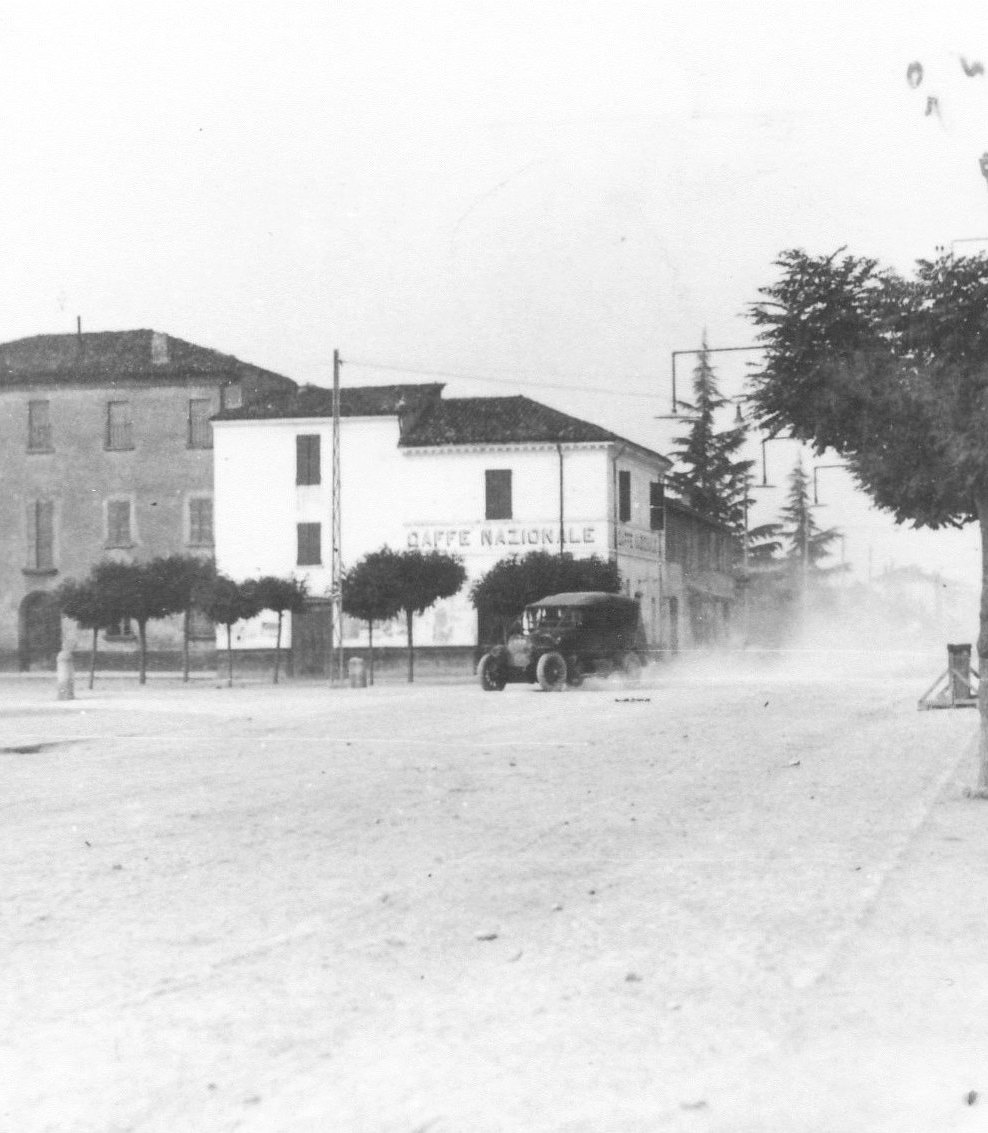
\includegraphics[width=\textwidth]{automobile}
    \caption[Automobile in piazza Monti]{Una delle prime automobili ad Alfonsine, in \index[Luoghi]{Piazza Vincenzo Monti}Piazza Monti.\label{fig:automobile}}
    \vspace{-0.7cm}
\end{figure}



 \begin{figure}[htb]
    \centering
    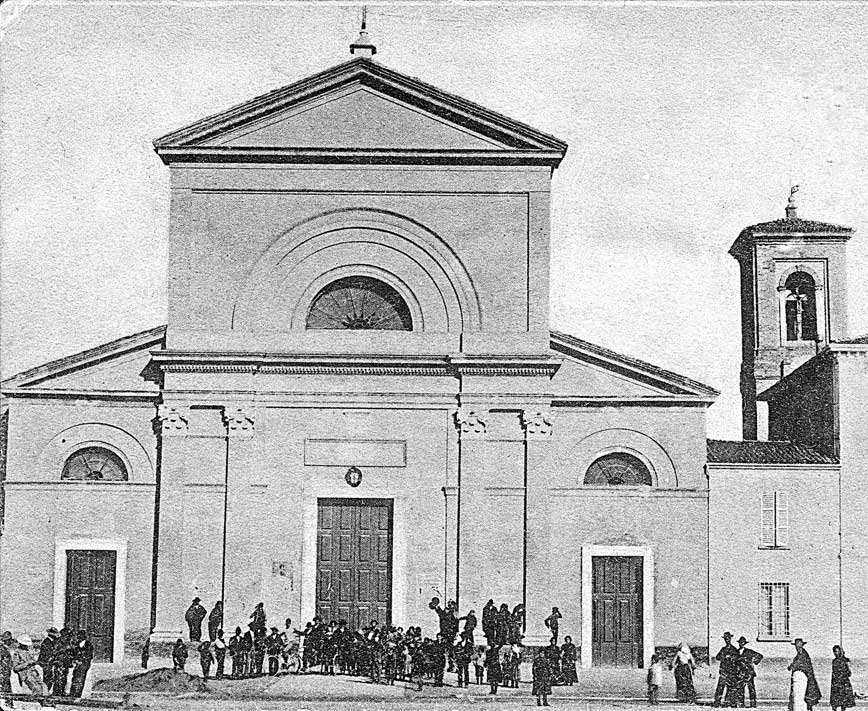
\includegraphics[width=\textwidth]{santamariafacciata}
    \caption{Facciata della chiesa Arcipretale Santa Maria\label{fig:santamariafacciata}}
    \vspace{-0.5cm}
\end{figure}





































%